\subsection{CodingJob: Um jogo sério para auxiliar nas disciplinas de Linguagem de Programação C}

Esta dissertação apresenta o jogo \textit{CodingJob}, um jogo sério que fornece um ambiente para prática dos conhecimentos da disciplina de \textit{Linguagem e Programação I} utilizando a linguagem C, não abrangindo nenhum conceito de Estruturas de Dados. Este é um jogo puzzle que apresenta desafios de programação, simulando um ambiente de trabalho, o objetivo é arrumar as secções de códigos necessárias. O conteudo didático deste é ensinado de forma explicita. \cite{costa2023condigjob}

\fixme{escrever sobre a conclusão do trabalho}

\begin{figure}[H]
	\centering
	\caption{Captura de tela do jogo CodingJob}
	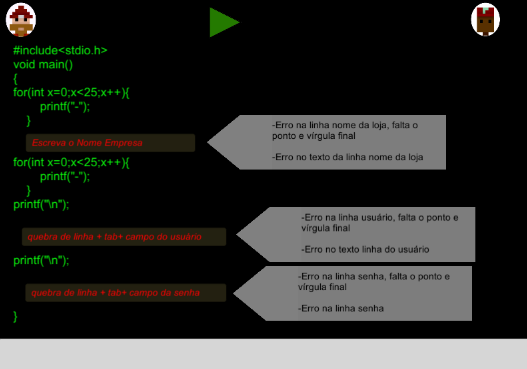
\includegraphics[width=0.8\textwidth]{images/codingjob.png}
	\legend{Fonte: \cite{costa2023condigjob}}
	\label{fig:codingjob}
\end{figure}

